% id: 130-h5
% book: 개념원리 중학 3-2 · 13 상자그림
% section: 핵심문제 익히기
% figure: crop:fig-130-h5.png
% answer: ㄴ, ㄷ
% answer_source: 본문 답
% variant_level: 0 (원본 전사)
% 이 파일은 build.mjs 가 items.json 에서 만든다. 고칠 때는 items.json 을 고친다.
\smash{\raisebox{1.5mm}{\dmkichul{개념원리 중학 3-2 130쪽 핵심문제 5}}}
\noindent\begin{minipage}[t]{0.58\linewidth}\vspace{0pt}\raggedright 오른쪽 그림은 $\pt{A}$, $\pt{B}$ 두 반 학생들의 영어 성적을 조사하여 나타낸 상자그림이다. 다음 \textbf{보기} 중 옳은 것을 모두 고르시오.\end{minipage}\hfill\begin{minipage}[t]{0.4\linewidth}\vspace{0pt}\centering \setlength{\dmfigw}{181.2pt}\ifdim\dmfigw>\linewidth\setlength{\dmfigw}{\linewidth}\fi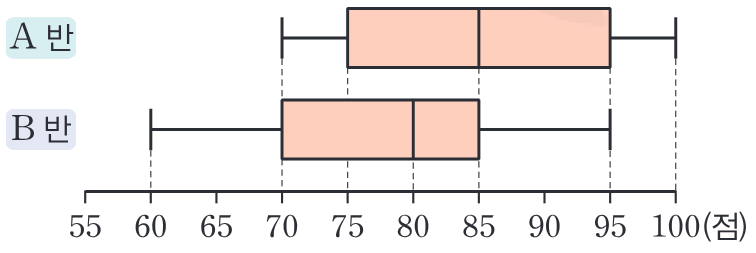
\includegraphics[width=\dmfigw]{figures/fig-130-h5.png}\end{minipage}\par
\noindent \bogi{ㄱ. $\pt{A}$ 반과 $\pt{B}$ 반의 영어 성적의 중앙값은 같다.\\ ㄴ. $\pt{A}$ 반과 $\pt{B}$ 반 전체에서 영어 성적이 가장 낮은 학생은 $\pt{B}$ 반에 있다.\\ ㄷ. $\pt{A}$ 반의 영어 성적이 $\pt{B}$ 반의 영어 성적보다 대체로 높다고 할 수 있다.}
